\section{Introduction}

Search Agents issue queries, inspect selected results, and reformulate their information need over long horizons. Their traces are therefore an attractive source of retriever supervision: a visited document can become a positive and surfaced-but-unvisited results can populate a negative pool~\cite{zhou2026lrat}. The latter operation is convenient, but behavior is not a relevance judgment. A result can remain unvisited because it is irrelevant, redundant with evidence already found, overlooked by the policy, or deferred until a later search step.

We ask: \emph{when is a retrieved but unvisited result a reliable training negative?} We answer this as a measurement question before attempting a new training rule. Using the official trajectories released with a recent study of long-horizon search behavior~\cite{liu2026diagnosing}, we reconstruct 638,215 ranked candidate occurrences from six Agents on the 830-question BrowseComp-Plus benchmark~\cite{chen2025browsecompplus}. We align every trajectory to evidence and gold qrels by exact normalized question text and preserve repeated exposures rather than prematurely collapsing a query--document pair.

Our audit gives three findings. First, 13.77\% of unvisited candidate occurrences belong to the evidence qrels; the mean within-query rate is 19.69\%, showing that long trajectories materially affect the pooled estimand. Second, the label is highly conditional. A candidate visited only after a later search is evidence-relevant 66.69\% of the time, versus 12.14\% otherwise. The contrast remains 67.99 percentage points when restricted to first exposures. Repeated results, high ranks, late search, and accumulated evidence also have substantially higher rates. Third, a conservative pre-registered coverage gate stops the training intervention: although all questions and all recoverable successful searches map, only 98.88\% of successful visits map back to a surfaced candidate, below the 99\% gate. The missingness is concentrated in one Agent. We therefore report a diagnostic result and a falsified method-readiness decision, not a post-hoc training gain.

\section{Related Work}

LRAT derives retriever pairs from Agent searches, document visits, and subsequent reasoning~\cite{zhou2026lrat}. It establishes that trajectories can provide useful supervision; our target is narrower and complementary: the conditional qrel reliability of documents eligible to become negatives. Diagnosing Search Behavior separates retrieval from evidence utilization across long-horizon Agents~\cite{liu2026diagnosing}. We reuse its released trajectories and state-oriented diagnostic style, but our outcome is the training label attached before model fitting rather than end-to-end failure attribution.

Behavioral supervision also resembles learning from logged clicks, where an unobserved action combines relevance with exposure and examination policy~\cite{joachims2017unbiased}. Agent traces differ because the policy actively reformulates queries, observes snippets, and may revisit a document after its information state changes. This makes rank correction alone insufficient and motivates conditioning on search progress, accumulated evidence, repeated retrieval, and cross-Agent agreement.

\section{Data and Candidate Reconstruction}

\paragraph{Trajectories and qrels.}
The released dataset contains one complete trajectory for each of six Agents and each BrowseComp-Plus question (4,980 trajectories). All runs use the same fixed corpus, Qwen3-Embedding-8B retriever, and top-$5$ search interface. BrowseComp-Plus provides broad \emph{evidence} qrels and stricter \emph{gold} qrels that are sufficient to answer the question~\cite{chen2025browsecompplus}. Evidence membership is our primary relevance outcome. Absence from the qrels is interpreted according to the benchmark evaluation protocol, not as proof of universal irrelevance.

\paragraph{Event semantics.}
For candidate occurrence $i$, let $S_i=1$ denote appearance in a search result and $V_i=1$ denote a successful visit after that search but before the next search observation. A \emph{later visit} occurs after at least one intervening search. We retain rank, normalized search progress, evidence qrels already surfaced, prior exposures, Agent, and termination state. Failed tool calls are recorded but never converted into candidates or visits. Reasoning utilization is not directly observable and remains missing rather than being inferred from a visit.

Our primary estimand for context $x$ is
\begin{equation}
  p_x=P(R^{\mathrm{evid}}=1\mid S=1,V=0,x),
  \label{eq:relevance}
\end{equation}
where $R^{\mathrm{evid}}$ is evidence-qrel membership. We report a pooled candidate rate and, as a robustness check, the mean of within-query rates. Confidence intervals use 10,000 nonparametric bootstrap samples with the question as the resampling cluster; candidate occurrences from the same question are never treated as independent.

\begin{table}[t]
  \caption{Candidate reconstruction. Search recovery excludes explicitly failed or invalid requests.}
  \label{tab:coverage}
  \centering
  \small
  \begin{tabular}{lrr}
    \toprule
    Check & Count & Rate \\
    \midrule
    Question--run mappings & 4,980 / 4,980 & 100.00\% \\
    Successful search lists & 127,591 / 127,591 & 100.00\% \\
    Parsed visit arguments & 9,796 / 9,807 & 99.89\% \\
    Successful visit mappings & 8,587 / 8,684 & 98.88\% \\
    Candidate occurrences & \multicolumn{2}{r}{638,215} \\
    \bottomrule
  \end{tabular}
\end{table}

\paragraph{Coverage audit.}
All six files match the release manifest in file size, hash, row count, and termination counts. We map 4,980/4,980 questions and parse all 127,591 successful search lists. The logs also contain 2,661 invalid search calls and nine local failures, which have no result list. Of 9,807 visit calls, 1,123 fail; among 8,684 successful visits, 97 cannot be linked to any recovered candidate in that trajectory. Visit mapping is 100\% for DeepSeek-V4-Pro and GLM-5.1, 99.90\% for Kimi-K2.6, 99.85\% for Qwen3.5, 98.95\% for GPT-OSS, and 96.25\% for Tongyi-DR. This concentration motivates the coverage gate rather than silent imputation.

\begin{figure}[t]
  \centering
  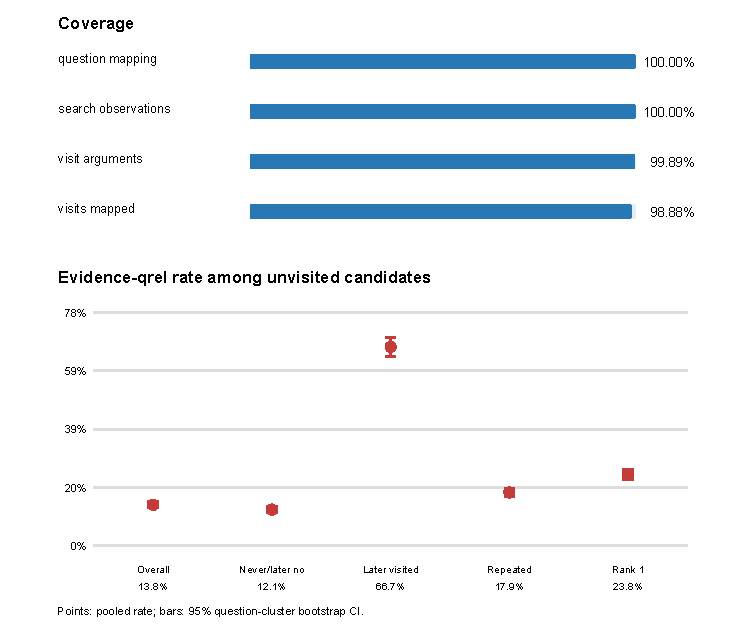
\includegraphics[width=\columnwidth]{../../analysis/negative_reliability/coverage_reliability_column.pdf}
  \caption{Reconstruction coverage and selected evidence-qrel rates among candidates unvisited before the next search. Error bars are 95\% question-cluster bootstrap intervals.}
  \Description{Four compact coverage bars above five point estimates with confidence intervals for overall, later-visit, repeated-retrieval, and rank-one candidate groups.}
  \label{fig:audit}
\end{figure}

\section{Negative Reliability Audit}

\subsection{Unvisited does not mean irrelevant}

Among 633,083 unvisited candidate occurrences, 87,168 (13.77\%, 95\% CI [12.81, 14.74]) are evidence-qrel positives. The query-balanced estimate is higher: 19.69\% [18.49, 20.89]. Under the stricter gold qrels, the corresponding pooled rate is 6.75\% [6.17, 7.37]. Thus even the global label has nontrivial benchmark-positive contamination, while the exact magnitude depends on whether each exposure or each question receives equal weight.

\subsection{Behavior exposes strong heterogeneity}

Table~\ref{tab:conditions} shows the pre-specified slices. Later-visited candidates have an evidence-qrel rate of 66.69\%, versus 12.14\% for candidates never visited later, a difference of 54.54 points [51.66, 57.43]. This is not only a repetition artifact: on first exposure, the later-visit rate is 73.79\%, versus 5.79\%, a difference of 68.00 points [65.87, 70.11]. Gold-qrel membership gives the same direction (44.55\% versus 2.56\% on first exposure).

Repeated retrieval is also informative. Its evidence rate is 17.89\%, compared with 7.21\% on first exposure. Excluding every later-visited occurrence, the repeated-minus-first contrast remains 10.40 points [9.41, 11.45]. Cross-Agent agreement is stronger still: documents surfaced by five or six Agents exceed documents surfaced by one Agent by 22.76 points [20.88, 24.69]. These outcomes ground behavioral stability signals in human qrels without calling behavior itself ground truth.

\begin{table}[t]
  \caption{Evidence-qrel rate among unvisited candidate occurrences. All intervals resample questions.}
  \label{tab:conditions}
  \centering
  \small
  \begin{tabular}{lrr}
    \toprule
    Condition & Candidates & Rate [95\% CI] \\
    \midrule
    Overall & 633,083 & 13.77 [12.81, 14.74] \\
    Later visited: no & 614,217 & 12.14 [11.29, 13.02] \\
    Later visited: yes & 18,866 & 66.69 [63.49, 69.96] \\
    First exposure only & 244,322 & 7.21 [6.76, 7.68] \\
    Repeated retrieval & 388,761 & 17.89 [16.59, 19.27] \\
    Rank 1 & 125,279 & 23.77 [22.15, 25.47] \\
    Rank 3--5 & 381,240 & 9.62 [8.87, 10.40] \\
    Early search & 196,484 & 9.24 [8.43, 10.08] \\
    Late search & 222,298 & 18.31 [17.19, 19.52] \\
    No prior evidence & 263,886 & 2.03 [1.82, 2.26] \\
    Complete prior evidence & 55,084 & 35.86 [33.03, 38.81] \\
    \bottomrule
  \end{tabular}
\end{table}

Rank and search state provide complementary structure. Rank-1 candidates are evidence-relevant 23.77\% of the time, versus 9.62\% at ranks 3--5. Rates rise from 9.24\% in the first third of search to 18.31\% in the final third. They also rise from 2.03\% before any evidence qrel has surfaced to 35.86\% after all evidence qrels have already surfaced. The last pattern is compatible with redundancy or attention limits, not merely with lack of evidence.

All six Agents show the same nonzero phenomenon, with overall evidence rates from 11.97\% to 16.21\%. Query difficulty changes the base rate: questions for which zero or one Agent ever surfaces a gold document have a 2.96\% unvisited evidence rate, while questions with five or six successful Agents reach 22.17\%. These are descriptive strata; difficulty is defined from cross-Agent retrieval and is not an independent causal variable.

\section{Gate, Existing Training Evidence, and Scope}

Before analysis, we required complete six-Agent question coverage, at least 99\% recovery of search/visit fields and successful-visit mappings, and a behavior-conditioned difference of at least 0.5 points whose question-bootstrap interval excludes zero. The signal criterion passes by a wide margin, as do question, search, and visit-argument recovery. Successful-visit mapping is 98.88\%, so the joint gate returns \textsc{Pivot}. We do not lower the threshold after observing strong curves and do not run a retriever intervention.

This decision also prevents an invalid shortcut through earlier LRAT experiments. The diagnostic trajectories use BrowseComp-Plus questions, whereas the released LRAT training trajectories use InfoSeekQA seed questions. Numeric IDs overlap accidentally but question text does not; row-level qrel transfer is prohibited. Existing controlled experiments on the LRAT data show that reasoning-length weights vary by configuration and seed; key Dev1500 paired-bootstrap intervals cross zero. They supply infrastructure and a fixed split, but cannot turn the present association into a training mechanism.

If coverage is repaired in a future release, the pre-specified intervention is modest: remove a negative that is successfully visited later in the same trajectory, retain at least five negatives, and compare against per-row removal-count-matched random and repeated-exposure controls. Until then, the supported contribution is diagnostic: surfaced-but-unvisited candidates form a heterogeneous supervision source, and later behavior plus qrels can identify where the label is least trustworthy.

\section{Robustness and Reproducibility}

Three checks separate the main contrast from convenient definitions. First, stricter gold qrels reduce absolute rates but preserve direction: 40.19\% of later-visited candidates are gold positives, compared with 5.72\% otherwise. On first exposure the rates are 44.55\% and 2.56\%, respectively. Second, repetition remains informative after excluding all later visits: repeated exposures exceed first exposures by 10.40 evidence points and 5.19 gold points. Third, Agent-specific pooled evidence rates occupy a relatively narrow 11.97--16.21\% range even though tool reliability differs, so the global phenomenon is not created by the low-coverage Agent alone.

The full analysis is deterministic from a single occurrence-level table. Each row records the question and trajectory identifiers, Agent, search step and query, document ID, rank, score, immediate and later visit states, prior exposure count, evidence state, evidence/gold memberships, termination, and source dataset. The table contains no inferred utilization label. Construction checks all six source files against the official release manifest and joins questions by normalized text; this specifically prevents the accidental numeric-ID join to the unrelated LRAT trajectories.

Machine-readable files retain every denominator, planned contrast, bootstrap setting, and the gate result. The confidence procedure uses seed 20260820 and 10,000 query-cluster resamples. The plotting artifact is generated from the same summary rather than transcribed by hand. A separate local dry run reconstructs the LRAT query-disjoint 94,113-row training split and verifies 93,977 stable trajectory mappings, but its three count-matched arms remain untrained because the diagnostic gate fails. This preserves a reproducible next experiment without converting preparation into a reported result.

\section{Limitations and Conclusion}

Qrels operationalize benchmark relevance, not step-specific utility. A later visit may be caused by policy mistakes, repeated exposure, or changing information needs. Candidate occurrences overweight long trajectories in the pooled estimand, which is why we report query-balanced estimates. Tool-call failures and unmatched visits are Agent-dependent, and the 99\% gate intentionally treats this as a method-readiness failure. Finally, our six Agents share one corpus and retriever; magnitudes may change with another interface or retrieval model.

We conclude that absence of a visit is not a uniform negative label. Evidence-qrel rates vary by more than an order of magnitude across observable contexts, and the strongest contrasts survive first-exposure and gold-qrel checks. Equally important, a conservative gate prevents these diagnostic findings from being overextended into an unsupported method claim.

% Keep the author-visible demo at four pages in total: page four contains the
% unrestricted Ethical Considerations and references area.
\clearpage
